\newpage
\section{Zimny start}\label{chapter:results_cold_start}

Drugim badanym kryterium jest czas działania funkcji podczas zimnych startów, które wymagają odpowiedniej inicjaliacji funkcji.
Z reguły są one dłuższe niż ciepłe starty, co może szczególnie wpłynąć na ogólną wydajność \cite{9284261}\cite{8605777}.
Średni czas działania funkcji został przedstawiony na Rysunkach \ref{fig:avg_cold_start_128_256}, \ref{fig:avg_cold_start_512_2045} oraz w Tabeli \ref{table:cold_start_comparison}.
Funkcje zostały wywołane stukrotnie.

\begin{figure}[!h]
    \centering
    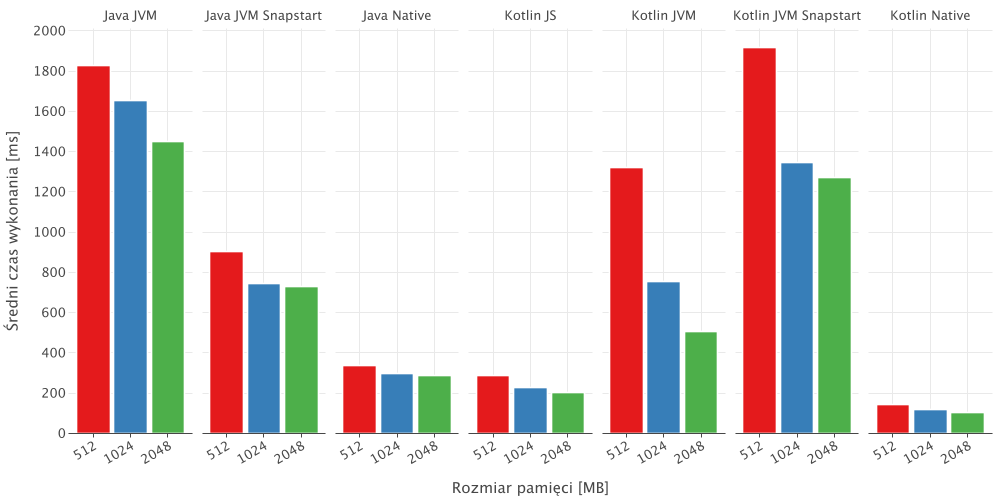
\includegraphics[width=0.95\textwidth]{charts/results/avg-cold-start-512-2048.png}
    \caption{Średni czas wykonywania funkcji (zimny start) dla rozmiarów pamięci: 512 MB, 1024 MB, 2048 MB  [źródło: opracowanie własne]}
    \label{fig:avg_cold_start_512_2045}
\end{figure}

Wpływ aktywacji usługi SnapStart jest różny w zależności od języka oprogramowania.
Dla Javy, usługa ta pozwoliła na poprawę czasu działania funkcji, w szczególności dla większych rozmiarów pamięci.
W przypadku języka Kotlin, jej aktywacja wpłynęła negatywnie na wydajność, wydłużając czas procesowania.
Samo użycie Kotlina (działającego w oparciu o JVM) pozwoliło na przyspieszenie obliczeń dla większych rozmiarów pamięci (512-2048 MB).

Znaczna poprawa wydajności została osiągnięte dla funkcji opartych o GraalVM oraz Kotlin/JS.
Obie metody uzyskały podobne wyniki, przy czym funkcja natywna GraalVM osiągnęła poprawę w przypadku rozmiarów pamięci 128 MB i 256 MB.
Dla wielkości 512-2048 MB, Kotlin/JS osiągnął niższe czasy działania niż funkcja GraalVM.
Niezależnie od rozmiaru pamięci najkrótszy czas działania w przypadku zimnego startu osiągnęły funkcje oparte o technologię Kotlin/Native.
Metoda ta pozwoliła także na osiągnięcie wyników o podobnej stabilności jak pozostałe funkcje, co zostało przedstawione na Rysunkach \ref{fig:warm_start_256} i \ref{fig:warm_start_1024}.
Mocno zróżnicowane wyniki zostały osiągnięte przez funkcję Kotlin z aktywowaną funkcją SnapStart.

\begin{table}[htbp]
\centering
\caption{Porównanie średnich, median oraz odchyleń standardowych czasów działania funkcji podczas zimnego startu względem funkcji bazowej (Java JVM) [źródło: opracowanie własne]}
\small
\begin{tabular}{|>{\centering\arraybackslash}m{2cm}|l|p{1.5cm}|p{1.5cm}|p{1.5cm}|p{1.5cm}|p{1.5cm}|}
\toprule
Rozmiar pamięci [MB] & Metoda & Średnia [ms] & Zmiana średniej & Mediana [ms] & Zmiana mediany & Odch. stand. \\
\midrule
\multirow{7}{*}{128} & Java JVM & 2725.84 & \mbox{0\%} & 2735.50 & \mbox{0\%} & 117.90 \\
 & Java GraalVM & 596.04 & \mbox{-78\%} & 600.22 & \mbox{-78\%} & 23.59 \\
 & Java JVM + SnapStart & 2465.93 & \mbox{-10\%} & 2473.31 & \mbox{-10\%} & 271.41 \\
 & Kotlin JVM & 4926.53 & \mbox{+81\%} & 4943.95 & \mbox{+81\%} & 200.56 \\
 & Kotlin JVM + SnapStart & 5853.27 & \mbox{+115\%} & 5937.41 & \mbox{+117\%} & 296.27 \\
 & Kotlin/JS & 679.17 & \mbox{-75\%} & 716.08 & \mbox{-74\%} & 110.08 \\
 & Kotlin/Native & 328.30 & \mbox{-88\%} & 323.46 & \mbox{-88\%} & 27.58 \\
\midrule
\multirow{7}{*}{256} & Java JVM & 2165.08 & \mbox{0\%} & 2196.40 & \mbox{0\%} & 109.60 \\
 & Java GraalVM & 416.56 & \mbox{-81\%} & 422.00 & \mbox{-81\%} & 19.06 \\
 & Java JVM + SnapStart & 1287.45 & \mbox{-41\%} & 1274.12 & \mbox{-42\%} & 200.26 \\
 & Kotlin JVM & 2426.35 & \mbox{+12\%} & 2449.18 & \mbox{+12\%} & 186.12 \\
 & Kotlin JVM + SnapStart & 3185.35 & \mbox{+47\%} & 3239.76 & \mbox{+48\%} & 234.01 \\
 & Kotlin/JS & 424.45 & \mbox{-80\%} & 430.08 & \mbox{-80\%} & 23.58 \\
 & Kotlin/Native & 204.49 & \mbox{-91\%} & 198.43 & \mbox{-91\%} & 25.21 \\
\midrule
\multirow{7}{*}{512} & Java JVM & 1826.74 & \mbox{0\%} & 1864.82 & \mbox{0\%} & 121.63 \\
 & Java GraalVM & 335.18 & \mbox{-82\%} & 343.65 & \mbox{-82\%} & 22.05 \\
 & Java JVM + SnapStart & 901.46 & \mbox{-51\%} & 887.57 & \mbox{-52\%} & 173.60 \\
 & Kotlin JVM & 1319.84 & \mbox{-28\%} & 1325.18 & \mbox{-29\%} & 71.54 \\
 & Kotlin JVM + SnapStart & 1915.50 & \mbox{+5\%} & 1997.87 & \mbox{+7\%} & 240.69 \\
 & Kotlin/JS & 286.63 & \mbox{-84\%} & 291.69 & \mbox{-84\%} & 20.85 \\
 & Kotlin/Native & 142.86 & \mbox{-92\%} & 135.35 & \mbox{-93\%} & 26.23 \\
\midrule
\multirow{7}{*}{1024} & Java JVM & 1651.76 & \mbox{0\%} & 1681.09 & \mbox{0\%} & 105.45 \\
 & Java GraalVM & 299.29 & \mbox{-82\%} & 307.39 & \mbox{-82\%} & 26.36 \\
 & Java JVM + SnapStart & 745.45 & \mbox{-55\%} & 719.96 & \mbox{-57\%} & 192.00 \\
 & Kotlin JVM & 754.19 & \mbox{-54\%} & 760.33 & \mbox{-55\%} & 58.38 \\
 & Kotlin JVM + SnapStart & 1346.78 & \mbox{-18\%} & 1417.63 & \mbox{-16\%} & 253.09 \\
 & Kotlin/JS & 227.63 & \mbox{-86\%} & 230.38 & \mbox{-86\%} & 17.27 \\
 & Kotlin/Native & 119.18 & \mbox{-93\%} & 108.99 & \mbox{-94\%} & 27.45 \\
\midrule
\multirow{7}{*}{2048} & Java JVM & 1450.35 & \mbox{0\%} & 1472.77 & \mbox{0\%} & 82.92 \\
 & Java GraalVM & 286.81 & \mbox{-80\%} & 297.54 & \mbox{-80\%} & 21.87 \\
 & Java JVM + SnapStart & 730.70 & \mbox{-50\%} & 712.26 & \mbox{-52\%} & 153.74 \\
 & Kotlin JVM & 504.26 & \mbox{-65\%} & 493.75 & \mbox{-66\%} & 63.05 \\
 & Kotlin JVM + SnapStart & 1272.25 & \mbox{-12\%} & 1351.34 & \mbox{-8\%} & 276.00 \\
 & Kotlin/JS & 201.25 & \mbox{-86\%} & 203.99 & \mbox{-86\%} & 12.08 \\
 & Kotlin/Native & 105.19 & \mbox{-93\%} & 99.50 & \mbox{-93\%} & 20.28 \\
\bottomrule
\end{tabular}
\label{tab:cold_start_comparison}
\end{table}

\begin{figure}[p] % Use [p] to suggest a float page. Or [!htbp] for more flexibility.
    \centering

    % --- First graphical element ---
    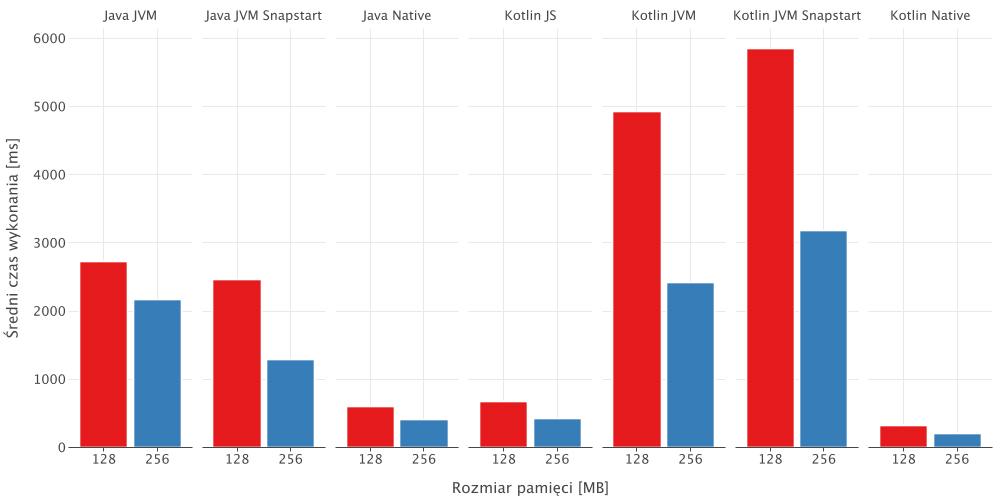
\includegraphics[width=0.95\textwidth]{charts/results/avg-cold-start-128-256.png}
    \caption{Średni czas wykonywania funkcji (zimny start) dla rozmiarów pamięci: 128 MB, 256 MB  [źródło: opracowanie własne]}
    \label{fig:avg_cold_start_128_256}

    \vspace{2em} % Optional: Add some vertical space between the distinct parts within this single figure

    % --- Second graphical element (with minipages) ---
    % Note: No new \begin{figure} here. This is part of the same float.
    \begin{minipage}[t]{0.48\textwidth}
        \centering
        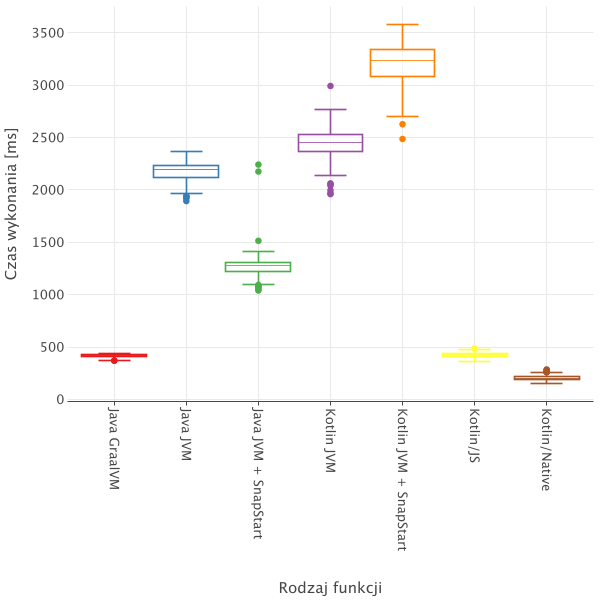
\includegraphics[width=\linewidth]{charts/results/cold-start-boxplot-256.png}
        \captionof{figure}{Czas wykonania funkcji (zimny start, 256 MB) [źródło: opracowanie własne]} % \captionof requires the 'caption' or 'capt-of' package
        \label{fig:cold_start_128}
    \end{minipage}% <--- % is important to prevent extra horizontal space
    \hfill % Creates flexible space between the minipages
    \begin{minipage}[t]{0.48\textwidth}
        \centering
        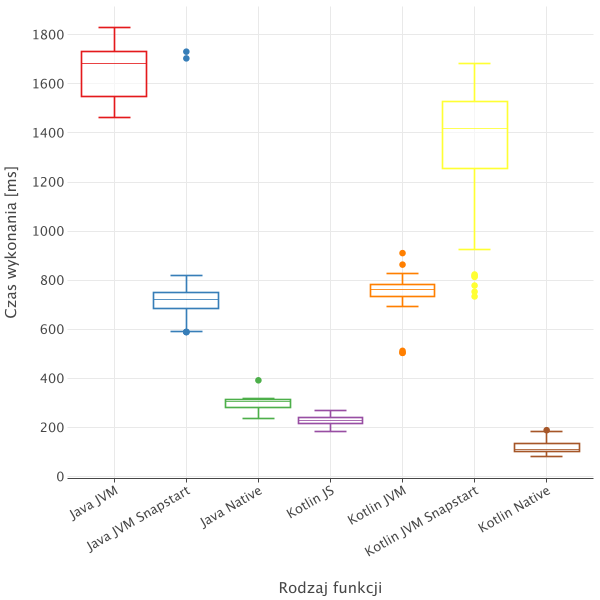
\includegraphics[width=\linewidth]{charts/results/cold-start-boxplot-1024.png}
        \captionof{figure}{Czas wykonania funkcji (zimny start, 1024 MB) [źródło: opracowanie własne]}
        \label{fig:cold_start_256}
    \end{minipage}
    % If this combined figure needs an overall caption, you could add another \caption{} here.
    % If the first caption serves as the overall caption, then this is fine.
\end{figure}
